\documentclass[11pt,a4paper]{report}
\usepackage[textwidth=37em,vmargin=30mm]{geometry}
\usepackage{calc,xunicode,amsmath,amssymb,paralist,enumitem,tabu,booktabs,datetime2,xeCJK,xeCJKfntef,listings}
\usepackage{tocloft,fancyhdr,tcolorbox,xcolor,graphicx,eso-pic,xltxtra,xelatexemoji}

\newcommand{\envyear}[0]{2025}
\newcommand{\envdatestr}[0]{2025-02-09}
\newcommand{\envfinaldir}[0]{webdb/2025/20250209/final}

\usepackage[hidelinks]{hyperref}
\hypersetup{
    colorlinks=false,
    pdfpagemode=FullScreen,
    pdftitle={Web Digest - \envdatestr}
}

\setlength{\cftbeforechapskip}{10pt}
\renewcommand{\cftchapfont}{\rmfamily\bfseries\large\raggedright}
\setlength{\cftbeforesecskip}{2pt}
\renewcommand{\cftsecfont}{\sffamily\small\raggedright}

\setdefaultleftmargin{2em}{2em}{1em}{1em}{1em}{1em}

\usepackage{xeCJK,xeCJKfntef}
\xeCJKsetup{PunctStyle=plain,RubberPunctSkip=false,CJKglue=\strut\hskip 0pt plus 0.1em minus 0.05em,CJKecglue=\strut\hskip 0.22em plus 0.2em}
\XeTeXlinebreaklocale "zh"
\XeTeXlinebreakskip = 0pt


\setmainfont{Brygada 1918}
\setromanfont{Brygada 1918}
\setsansfont{IBM Plex Sans}
\setmonofont{JetBrains Mono NL}
\setCJKmainfont{Noto Serif CJK SC}
\setCJKromanfont{Noto Serif CJK SC}
\setCJKsansfont{Noto Sans CJK SC}
\setCJKmonofont{Noto Sans CJK SC}

\setlength{\parindent}{0pt}
\setlength{\parskip}{8pt}
\linespread{1.15}

\lstset{
	basicstyle=\ttfamily\footnotesize,
	numbersep=5pt,
	backgroundcolor=\color{black!5},
	showspaces=false,
	showstringspaces=false,
	showtabs=false,
	tabsize=2,
	captionpos=b,
	breaklines=true,
	breakatwhitespace=true,
	breakautoindent=true,
	linewidth=\textwidth
}






\newcommand{\coverpic}[2]{
    % argv: itemurl, authorname
    Cover photo by #2~~(\href{#1}{#1})
}
\newcommand{\makeheader}[0]{
    \begin{titlepage}
        % \newgeometry{hmargin=15mm,tmargin=21mm,bmargin=12mm}
        \begin{center}
            
            \rmfamily\scshape
            \fontspec{BaskervilleF}
            \fontspec{Old Standard}
            \fontsize{59pt}{70pt}\selectfont
            WEB\hfill DIGEST
            
            \vfill
            % \vskip 30pt
            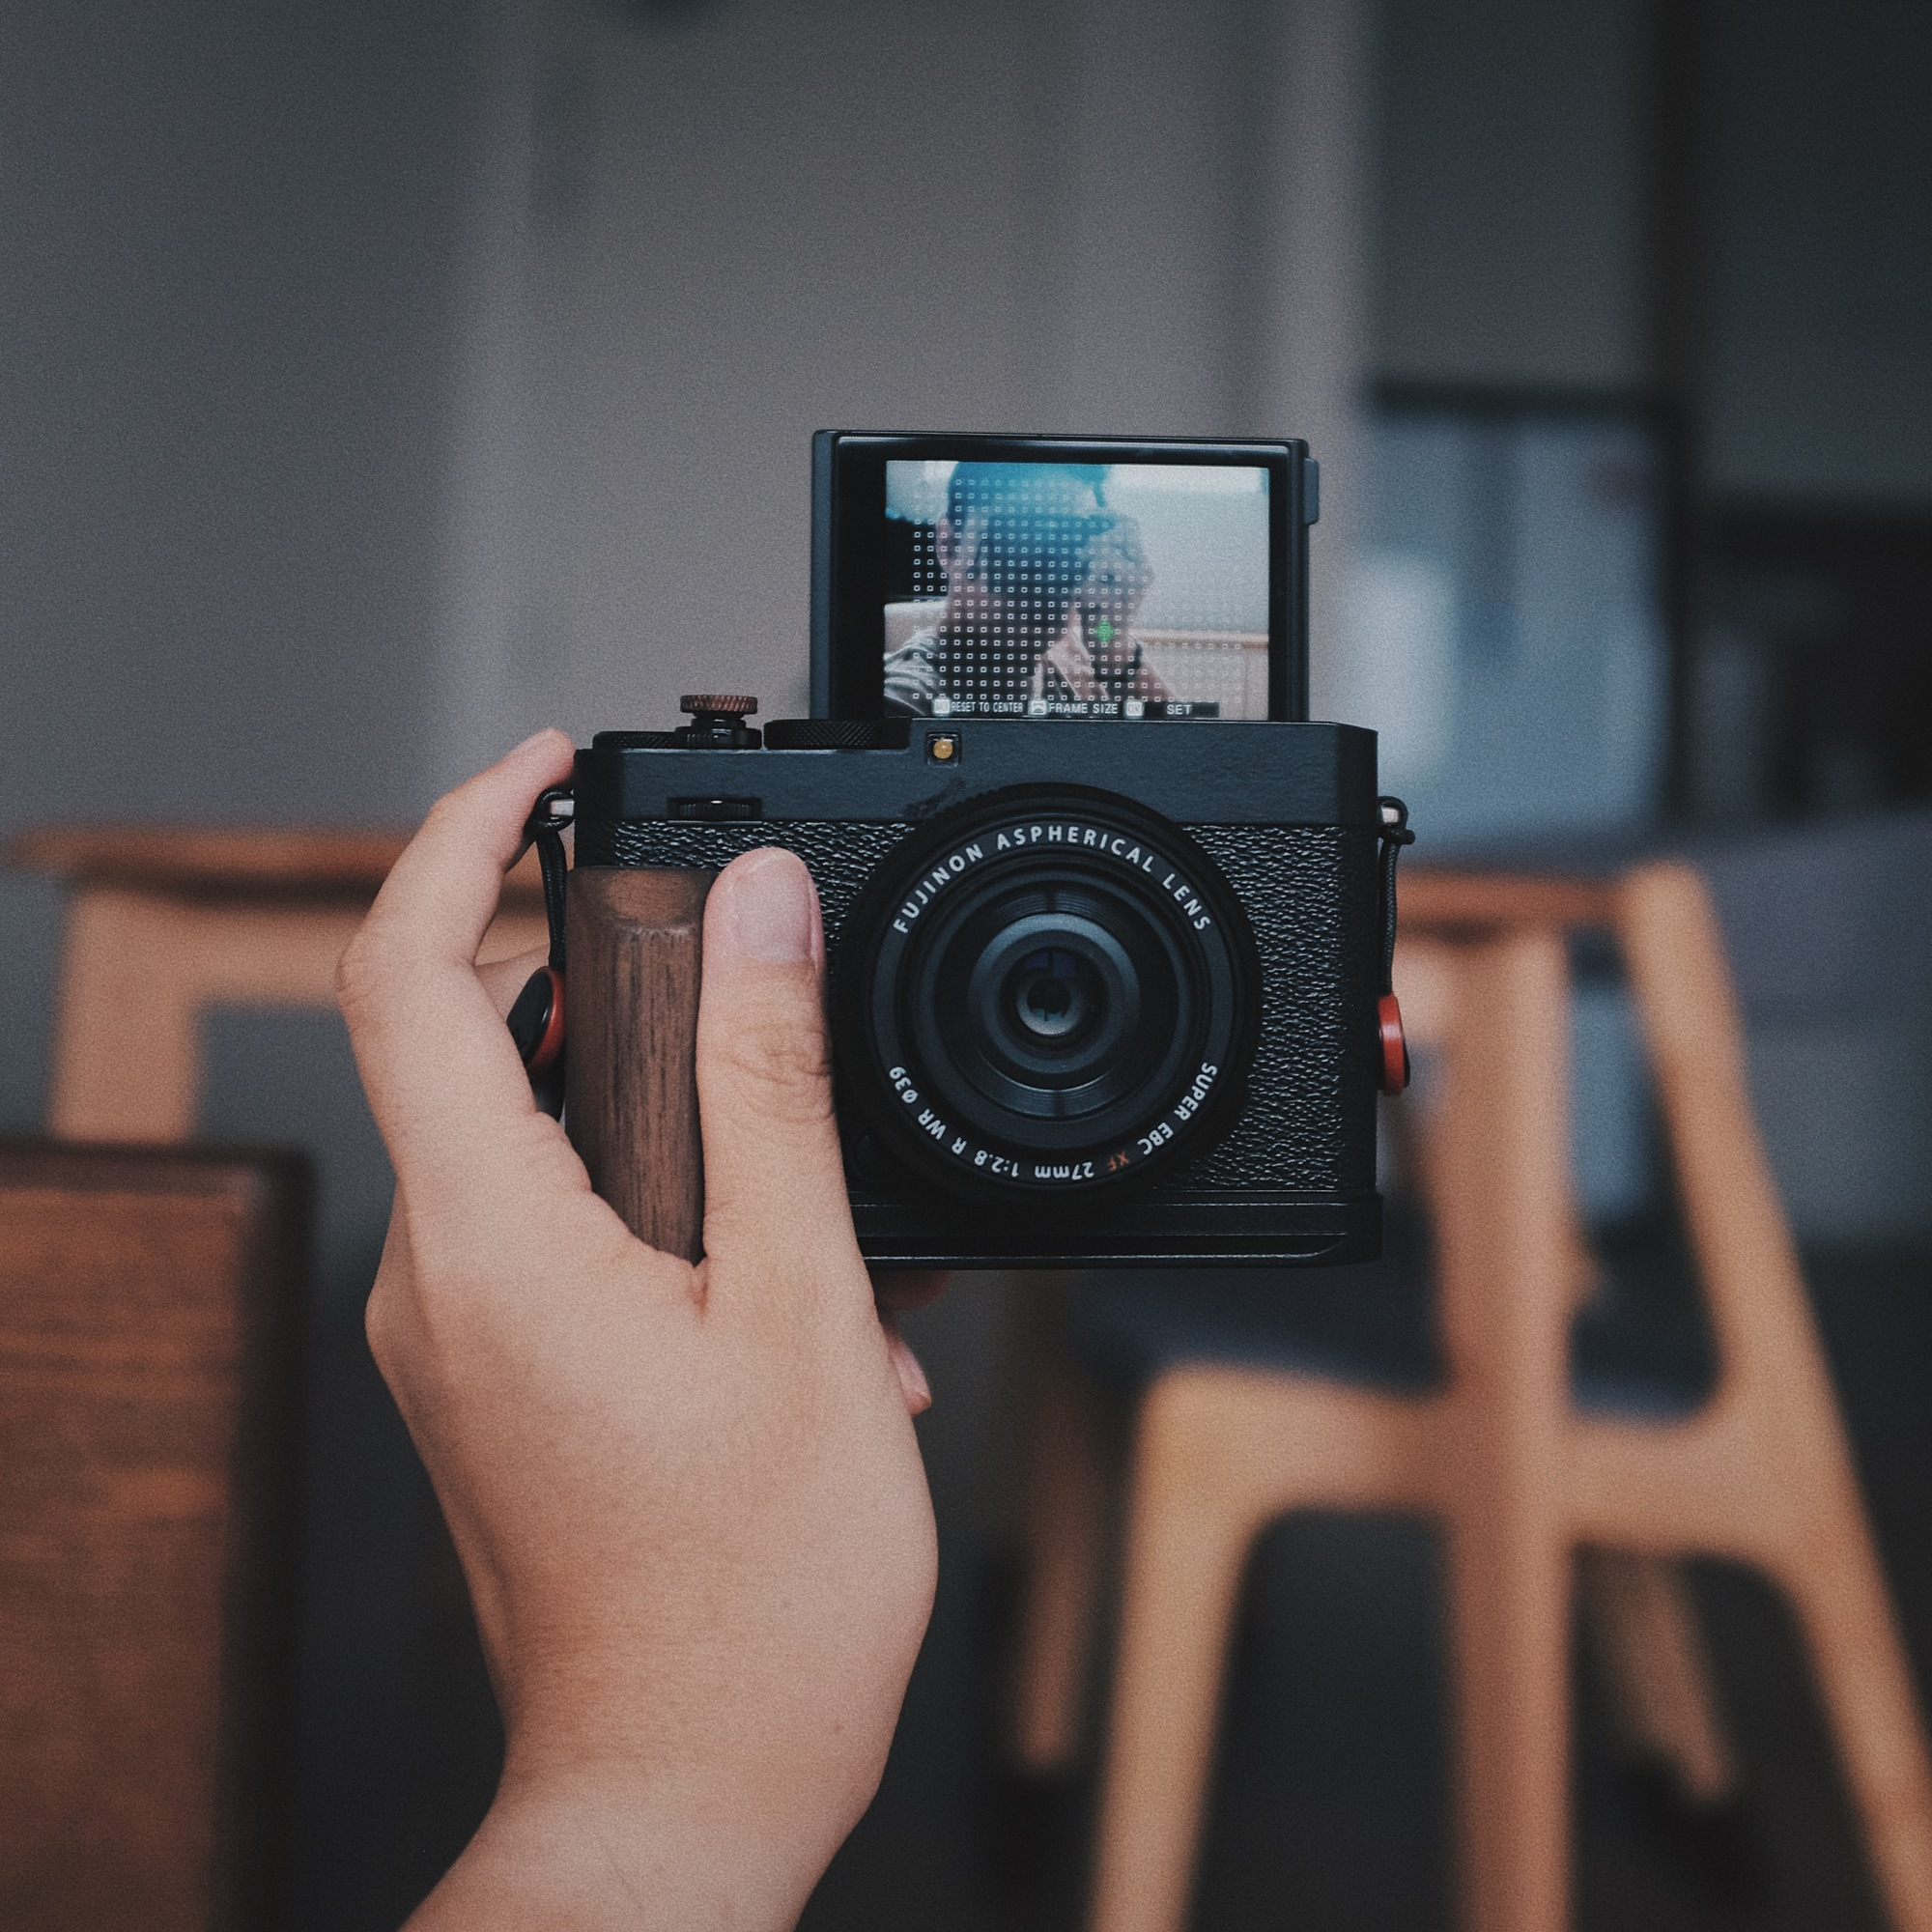
\includegraphics[width=\linewidth]{\envfinaldir/coverpic-prod.jpg}\par
            % \vskip 30pt
            \vfill

            \normalsize\rmfamily\scshape
            \copyright{} The Web Digest Project \hfill\large \envdatestr
        \end{center}
    \end{titlepage}
    % \restoregeometry
}
\newcommand{\simplehref}[1]{%
    \textcolor{blue!80!green}{\href{#1}{#1}}%
}
\renewcommand{\contentsname}{\center\Huge\sffamily\bfseries Contents\par\vskip 20pt}
\newcounter{ipartcounter}
\setcounter{ipartcounter}{0}
\newcommand{\ipart}[1]{
    % \vskip 20pt
    \clearpage
    \stepcounter{ipartcounter}
    \phantomsection
    \addcontentsline{toc}{chapter}{#1}
    % \begin{center}
    %     \Huge
    %     \sffamily\bfseries
    %     #1
    % \end{center}
    % \vskip 20pt plus 7pt
}
\newcounter{ichaptercounter}
\setcounter{ichaptercounter}{0}
\newcommand{\ichapter}[1]{
    % \vskip 20pt
    \clearpage
    \stepcounter{ichaptercounter}
    \phantomsection
    \addcontentsline{toc}{section}{\numberline{\arabic{ichaptercounter}}#1}
    \begin{center}
        \Huge
        \sffamily\bfseries
        #1
    \end{center}
    \vskip 20pt plus 7pt
}
\newcommand{\entrytitlefont}[1]{\subsection*{\raggedright\Large\sffamily\bfseries#1}}
\newcommand{\entryitemGeneric}[2]{
    % argv: title, url
    \parbox{\linewidth}{
        \entrytitlefont{#1}\par\vskip 5pt
        \footnotesize\ttfamily\mdseries
        \simplehref{#2}
    }\vskip 11pt plus 11pt minus 1pt
}
\newcommand{\entryitemGithub}[3]{
    % argv: title, url, desc
    \parbox{\linewidth}{
        \entrytitlefont{#1}\par\vskip 5pt
        \footnotesize\ttfamily\mdseries
        \simplehref{#2}\par\vskip 5pt
        \small\rmfamily\mdseries#3
    }\vskip 11pt plus 11pt minus 1pt
}
\newcommand{\entryitemAp}[3]{
    % argv: title, url, desc
    \parbox{\linewidth}{
        \entrytitlefont{#1}\par\vskip 5pt
        \footnotesize\ttfamily\mdseries
        \simplehref{#2}\par\vskip 5pt
        \small\rmfamily\mdseries#3
    }\vskip 11pt plus 11pt minus 1pt
}
\newcommand{\entryitemHackernews}[3]{
    % argv: title, hnurl, rawurl
    % \parbox{\linewidth}{
    %     \entrytitlefont{#1}\par\vskip 5pt
    %     \footnotesize\ttfamily\mdseries
    %     \simplehref{#3}\par
    %     \textcolor{black!50}{\href{#2}{#2}}
    % }\vskip 11pt plus 11pt minus 1pt
    \begin{minipage}{\linewidth}
            \entrytitlefont{#1}\par\vskip 5pt
            \footnotesize\ttfamily\mdseries
            \simplehref{#3}\par
            \textcolor{black!50}{\href{#2}{#2}}
    \end{minipage}\par\vskip 11pt plus 11pt minus 1pt
}







\begin{document}

\makeheader

\tableofcontents\clearpage




\ipart{Developers}
\ichapter{Hacker News}
\entryitemTwoLinks{Tips for mathematical handwriting (2007)}{https://news.ycombinator.com/item?id=42985427}{https://johnkerl.org/doc/ortho/ortho.html}

\entryitemTwoLinks{Writing a Simple Windows Driver in Rust}{https://news.ycombinator.com/item?id=42984457}{https://scorpiosoftware.net/2025/02/08/writing-a-simple-driver-in-rust/}

\entryitemTwoLinks{Show HN: FlashSpace – fast, open-source, macOS Spaces replacement}{https://news.ycombinator.com/item?id=42984420}{https://github.com/wojciech-kulik/FlashSpace}

\entryitemTwoLinks{Carbon is not a programming language (sort of)}{https://news.ycombinator.com/item?id=42983733}{https://herecomesthemoon.net/2025/02/carbon-is-not-a-language/}

\entryitemTwoLinks{The Deck: An open-source cross-platform multiplayer card game engine in Flutter}{https://news.ycombinator.com/item?id=42983699}{https://github.com/xajik/thedeck}

\entryitemTwoLinks{We are destroying software}{https://news.ycombinator.com/item?id=42983275}{https://antirez.com/news/145}

\entryitemTwoLinks{A tale of several distros joining forces for a common goal: reproducible builds}{https://news.ycombinator.com/item?id=42982270}{https://video.fosdem.org/2025/h1302/fosdem-2025-6479-a-tale-of-several-distros-joining-forces-for-a-common-goal-reproducible-builds.av1.webm}

\entryitemTwoLinks{Generating Voronoi Diagrams Using Fortune's Algorithm (With Odin)}{https://news.ycombinator.com/item?id=42982015}{https://redpenguin101.github.io/html/posts/2025\_01\_21\_voronoi.html}

\entryitemTwoLinks{LINUX is obsolete (1992)}{https://news.ycombinator.com/item?id=42980283}{https://groups.google.com/g/comp.os.minix/c/wlhw16QWltI}

\entryitemTwoLinks{Ghostwriter – use the reMarkable2 as an interface to vision-LLMs}{https://news.ycombinator.com/item?id=42979986}{https://github.com/awwaiid/ghostwriter}

\entryitemTwoLinks{Starlink in the Falkland Islands – A national emergency situation?}{https://news.ycombinator.com/item?id=42979869}{https://www.openfalklands.com/february-2025-starlink-in-the-falkland-islands-a-national-emergency-situation/}

\entryitemTwoLinks{VSCode's SSH agent is bananas}{https://news.ycombinator.com/item?id=42979467}{https://fly.io/blog/vscode-ssh-wtf/}

\entryitemTwoLinks{Obscure islands I find interesting}{https://news.ycombinator.com/item?id=42978199}{https://amanvir.com/obscure-islands}

\entryitemTwoLinks{Show HN: ExpenseOwl – Simple, self-hosted expense tracker}{https://news.ycombinator.com/item?id=42977388}{https://github.com/Tanq16/ExpenseOwl}

\entryitemTwoLinks{Do-nothing scripting: the key to gradual automation (2019)}{https://news.ycombinator.com/item?id=42976698}{https://blog.danslimmon.com/2019/07/15/do-nothing-scripting-the-key-to-gradual-automation/}

\entryitemTwoLinks{Show HN: A website that heatmaps your city based on your housing preferences}{https://news.ycombinator.com/item?id=42975803}{https://theretowhere.com/}

\entryitemTwoLinks{Cities can cost effectively start their own utilities}{https://news.ycombinator.com/item?id=42975492}{https://kevin.burke.dev/kevin/norcal-cities-new-utility/}

\entryitemTwoLinks{A brief history of code signing at Mozilla}{https://news.ycombinator.com/item?id=42975436}{https://hearsum.ca/posts/history-of-code-signing-at-mozilla/}

\entryitemTwoLinks{German civil activists win victory in election case against X}{https://news.ycombinator.com/item?id=42975170}{https://www.reuters.com/world/europe/german-civil-activists-claim-victory-case-against-musks-x-2025-02-07/}

\entryitemTwoLinks{Ketamine for Depression: How It Works (2024) [video]}{https://news.ycombinator.com/item?id=42974882}{https://www.yalemedicine.org/news/ketamine-for-depression}\ichapter{Phoronix}
\entryitemGeneric{\hskip 0pt{}SysVinit 3.14 Released: Overcomes Three Decade Limitation Of Inittab Line Length}{https://www.phoronix.com/news/SysVinit-3.14-Released}

\entryitemGeneric{\hskip 0pt{}Clang Thread Safety Checks Begin Uncovering Bugs In The Linux Kernel}{https://www.phoronix.com/news/Linux-Clang-Thread-Safety}

\entryitemGeneric{\hskip 0pt{}GNU G-Golf v0.8 Released For Writing GTK Apps In Guile/Scheme}{https://www.phoronix.com/news/GNU-G-Golf-0.8}

\entryitemGeneric{\hskip 0pt{}FEX 2502 Delivers Fix For Steam, Multi-Block Improvements For Better Performance}{https://www.phoronix.com/news/FEX-2502-Released}

\entryitemGeneric{\hskip 0pt{}KDE Plasma 6.3 Receives Final Polishing Prior To Release Next Week}{https://www.phoronix.com/news/KDE-Plasma-6.3-Next-Week}

\entryitemGeneric{\hskip 0pt{}FreeBSD 13.5 Beta Begins Preparing For The Last Of The FreeBSD 13 Series}{https://www.phoronix.com/news/FreeBSD-13.5-Beta-1-Released}

\entryitemGeneric{\hskip 0pt{}Wine 10.1 Released With Many Changes: Fixes For Battle.net, Continued Bluetooth Driver}{https://www.phoronix.com/news/Wine-10.1-Released}

\entryitemGeneric{\hskip 0pt{}GNOME's LocalSearch Metadata Extractor Ditches GStreamer For FFmpeg}{https://www.phoronix.com/news/GNOME-LocalSearch-FFmpeg}

\entryitemGeneric{\hskip 0pt{}IO\_uring Zero-Copy Receive Support Ready For Linux 6.15 Networking}{https://www.phoronix.com/news/IO\_uring-Zero-Copy-Receive-Net}\ichapter{Dribbble}
\entryitemGeneric{\hskip 0pt{}Barbershop POS app for booking and payments}{https://dribbble.com/shots/25596116-Barbershop-POS-app-for-booking-and-payments}

\entryitemGeneric{\hskip 0pt{}Seam Logo Redesigned}{https://dribbble.com/shots/25595119-Seam-Logo-Redesigned}

\entryitemGeneric{\hskip 0pt{}Cloaked Logo Design}{https://dribbble.com/shots/25585116-Cloaked-Logo-Design}

\entryitemGeneric{\hskip 0pt{}The Journey}{https://dribbble.com/shots/25590279-The-Journey}

\entryitemGeneric{\hskip 0pt{}CropBytes 2d \& 3d logo}{https://dribbble.com/shots/25590388-CropBytes-2d-3d-logo}

\entryitemGeneric{\hskip 0pt{}Wylder Logo Design - W letter monogram}{https://dribbble.com/shots/25589195-Wylder-Logo-Design-W-letter-monogram}

\entryitemGeneric{\hskip 0pt{}Easyalgos Logo Design}{https://dribbble.com/shots/25589439-Easyalgos-Logo-Design}

\entryitemGeneric{\hskip 0pt{}Carbon Solutions B2B Branding Design \& Visual Identity}{https://dribbble.com/shots/25525140-Carbon-Solutions-B2B-Branding-Design-Visual-Identity}

\entryitemGeneric{\hskip 0pt{}Dog / Puzzle Logo}{https://dribbble.com/shots/25581316-Dog-Puzzle-Logo}

\entryitemGeneric{\hskip 0pt{}Frank's Alley® Trailer \& Mascots}{https://dribbble.com/shots/25585516-Frank-s-Alley-Trailer-Mascots}

\entryitemGeneric{\hskip 0pt{}Glyph Beer Icons 51-62}{https://dribbble.com/shots/25585199-Glyph-Beer-Icons-51-62}

\entryitemGeneric{\hskip 0pt{}Chordio Chrome exstension}{https://dribbble.com/shots/25580857-Chordio-Chrome-exstension}

\entryitemGeneric{\hskip 0pt{}Realtree® 30 Years.}{https://dribbble.com/shots/25579343-Realtree-30-Years}

\entryitemGeneric{\hskip 0pt{}VCC Logo Design Vector Sketches}{https://dribbble.com/shots/25577220-VCC-Logo-Design-Vector-Sketches}

\entryitemGeneric{\hskip 0pt{}Brand Family System Loop}{https://dribbble.com/shots/25579103-Brand-Family-System-Loop}

\entryitemGeneric{\hskip 0pt{}Chilbot Motion Design}{https://dribbble.com/shots/25578623-Chilbot-Motion-Design}

\entryitemGeneric{\hskip 0pt{}Weve Branding}{https://dribbble.com/shots/25579635-Weve-Branding}

\entryitemGeneric{\hskip 0pt{}S}{https://dribbble.com/shots/25571540-S}

\entryitemGeneric{\hskip 0pt{}Fly Fry}{https://dribbble.com/shots/25573635-Fly-Fry}

\entryitemGeneric{\hskip 0pt{}Logo and Branding for VCC}{https://dribbble.com/shots/25571598-Logo-and-Branding-for-VCC}

\entryitemGeneric{\hskip 0pt{}Axolotl Mascot}{https://dribbble.com/shots/25572670-Axolotl-Mascot}

\entryitemGeneric{\hskip 0pt{}Finance APP UI Design}{https://dribbble.com/shots/25570740-Finance-APP-UI-Design}

\entryitemGeneric{\hskip 0pt{}TIAA Duotone Icons}{https://dribbble.com/shots/25573874-TIAA-Duotone-Icons}

\entryitemGeneric{\hskip 0pt{}Cloud Animation Sound Design}{https://dribbble.com/shots/25571319-Cloud-Animation-Sound-Design}


\ipart{Developers~~~~(zh-Hans)}
\ichapter{Solidot}
\entryitemGeneric{\hskip 0pt{}波音在 Starliner 项目上总损失超过了 20 亿美元}{https://www.solidot.org/story?sid=80504}

\entryitemGeneric{\hskip 0pt{}法国铁路对开扬声器打电话的乘客罚款 150 欧元}{https://www.solidot.org/story?sid=80503}

\entryitemGeneric{\hskip 0pt{}印度将推出银行专用域名 .bank.in}{https://www.solidot.org/story?sid=80502}

\entryitemGeneric{\hskip 0pt{}Microsoft 365 订阅费用准备涨价}{https://www.solidot.org/story?sid=80501}

\entryitemGeneric{\hskip 0pt{}Meta 从盗版电子书库下载了逾百 TB 的电子书}{https://www.solidot.org/story?sid=80500}

\entryitemGeneric{\hskip 0pt{}由于维护者拒绝 DMA Rust 抽象 Hector Martin 宣布退出内核开发}{https://www.solidot.org/story?sid=80499}

\entryitemGeneric{\hskip 0pt{}扩展开发者称 Google 没有信守在宣布 Manifest V3 时许下的承诺}{https://www.solidot.org/story?sid=80498}

\entryitemGeneric{\hskip 0pt{}英国政府命令苹果创建 iCloud 加密后门}{https://www.solidot.org/story?sid=80497}

\entryitemGeneric{\hskip 0pt{}Goolge 修复正被利用的 Android 内核 0day 漏洞}{https://www.solidot.org/story?sid=80496}

\entryitemGeneric{\hskip 0pt{}相信外星人的上世纪硅谷高管面临监禁}{https://www.solidot.org/story?sid=80495}

\entryitemGeneric{\hskip 0pt{}科学家声称找到煮鸡蛋的完美方法}{https://www.solidot.org/story?sid=80494}

\entryitemGeneric{\hskip 0pt{}2024 年勒索软件付款额下降 35\%}{https://www.solidot.org/story?sid=80493}

\entryitemGeneric{\hskip 0pt{}美国分析师认为 DeepSeek 的 AI App 有很高的可能性被禁}{https://www.solidot.org/story?sid=80492}

\entryitemGeneric{\hskip 0pt{}空气污染会影响日常工作的专注力}{https://www.solidot.org/story?sid=80491}

\entryitemGeneric{\hskip 0pt{}鲸歌的沟通效率与人类相似}{https://www.solidot.org/story?sid=80490}

\entryitemGeneric{\hskip 0pt{}研究人员提出一种超低成本的 AI 训练方法}{https://www.solidot.org/story?sid=80489}

\entryitemGeneric{\hskip 0pt{}北极气温上周日超过平均水平 20 摄氏度}{https://www.solidot.org/story?sid=80488}

\entryitemGeneric{\hskip 0pt{}苹果面临反垄断调查}{https://www.solidot.org/story?sid=80487}

\entryitemGeneric{\hskip 0pt{}OpenWrt 24.10 释出}{https://www.solidot.org/story?sid=80486}

\entryitemGeneric{\hskip 0pt{}iPhone 在华销量大幅下挫}{https://www.solidot.org/story?sid=80485}\ichapter{V2EX}
\entryitemGeneric{\hskip 0pt{}[宽带症候群] 请教一下, 在不购买跨境专线/SD-WAN 的情况下, 企业跨境站点互联怎么做比较合适?}{https://www.v2ex.com/t/1110041}

\entryitemGeneric{\hskip 0pt{}[程序员] 有什么类似 toby 的平替插件?}{https://www.v2ex.com/t/1110040}

\entryitemGeneric{\hskip 0pt{}[InfluxDB] InfluxDB 3 Open Source Now in Public Alpha Under MIT/Apache 2 License}{https://www.v2ex.com/t/1110039}

\entryitemGeneric{\hskip 0pt{}[问与答] orbstack 不支持动态内核}{https://www.v2ex.com/t/1110038}

\entryitemGeneric{\hskip 0pt{}[程序员] 组件化 Tailwind 传递 ClassName 参数最佳实践求解答}{https://www.v2ex.com/t/1110037}

\entryitemGeneric{\hskip 0pt{}[分享创造] 分享下用 DeepSeek R1 来写了这篇关于这款在线 AI 工具工具箱的文章}{https://www.v2ex.com/t/1110036}

\entryitemGeneric{\hskip 0pt{}[分享发现] [分享]做了个 X 的 AI 简中推文网页|求推荐优质的博主}{https://www.v2ex.com/t/1110035}

\entryitemGeneric{\hskip 0pt{}[问与答] 求助求助!在国内如何向 GCash 转账}{https://www.v2ex.com/t/1110033}

\entryitemGeneric{\hskip 0pt{}[硬件] hdmi 和 dp 的显色会不同吗?}{https://www.v2ex.com/t/1110032}

\entryitemGeneric{\hskip 0pt{}[问与答] 关于 clash verge 使用 proxy-providers 导入订阅链接报错 400 的疑问。}{https://www.v2ex.com/t/1110031}

\entryitemGeneric{\hskip 0pt{}[分享发现] 2025 年上架 Google play 踩坑记录}{https://www.v2ex.com/t/1110030}

\entryitemGeneric{\hskip 0pt{}[问与答] 如何在长辈来的几天让电视免费收看央视及地方卫视直播频道?求优雅方案}{https://www.v2ex.com/t/1110029}

\entryitemGeneric{\hskip 0pt{}[问与答] 家庭自用机柜选什么?}{https://www.v2ex.com/t/1110028}

\entryitemGeneric{\hskip 0pt{}[职场话题] 如何处理远程办公的情绪问题}{https://www.v2ex.com/t/1110027}

\entryitemGeneric{\hskip 0pt{}[分享创造] 新作 [词语乱序工具] ,帮助你自由发言!}{https://www.v2ex.com/t/1110026}

\entryitemGeneric{\hskip 0pt{}[Mac mini] 如何判断 mac mini 是否在睡眠中}{https://www.v2ex.com/t/1110025}

\entryitemGeneric{\hskip 0pt{}[问与答] 能否在 macOS 上实现只 AirPlay QQ 音乐的声音到音箱, 而不是将这个系统的声音全部 AirPlay 过去}{https://www.v2ex.com/t/1110024}

\entryitemGeneric{\hskip 0pt{}[问与答] 关于深圳道路没有规划非机动车道这件事}{https://www.v2ex.com/t/1110023}

\entryitemGeneric{\hskip 0pt{}[硬件] 不懂色彩管理,有个 LG 4K 显示器,之前一直用显示器自带的 LG 4K 颜色管理配置,现在换成了 display P3,颜色变淡了,饱和度稍低}{https://www.v2ex.com/t/1110022}

\entryitemGeneric{\hskip 0pt{}[问与答] scrum master 的工作内容能饱和吗 相当于监工}{https://www.v2ex.com/t/1110021}

\entryitemGeneric{\hskip 0pt{}[问与答] 求推荐一个敲击不费力的键盘}{https://www.v2ex.com/t/1110019}

\entryitemGeneric{\hskip 0pt{}[OpenAI] 付费使用 ChatGPT Pro 会员的一些体验}{https://www.v2ex.com/t/1110018}

\entryitemGeneric{\hskip 0pt{}[上海] 求指导卧室家具摆放设计}{https://www.v2ex.com/t/1110015}

\entryitemGeneric{\hskip 0pt{}[分享创造] 用 DeepSeek-r1 肝了一个看博客文章的 ios App,目前还处于开发与测试阶段,已经发了 Testflight,🙈大家给点建议!}{https://www.v2ex.com/t/1110013}

\entryitemGeneric{\hskip 0pt{}[分享创造] 使用 Rust + wgpu 创作的音画互动 / 动态壁纸 App 上线 App Store / Steam 啦,欢迎体验支持!}{https://www.v2ex.com/t/1110012}

\entryitemGeneric{\hskip 0pt{}[随想] 在 b 站看到一个门口安了监控拍到邻居的视频}{https://www.v2ex.com/t/1110010}

\entryitemGeneric{\hskip 0pt{}[问与答] 目前最真实的聊天模型是什么}{https://www.v2ex.com/t/1110009}

\entryitemGeneric{\hskip 0pt{}[投资] 最近有在中行(BOC)购汇并汇款到香港(美元)的 V 友吗,你们有遇到限制吗?}{https://www.v2ex.com/t/1110008}

\entryitemGeneric{\hskip 0pt{}[Apple TV] 又来发码了 tvOS / iOS 通用}{https://www.v2ex.com/t/1110007}

\entryitemGeneric{\hskip 0pt{}[分享创造] 肝了一个图片翻译的工具,大家看看}{https://www.v2ex.com/t/1110005}

\entryitemGeneric{\hskip 0pt{}[问与答] 老生常谈,腾讯会议的平替有什么?}{https://www.v2ex.com/t/1110004}

\entryitemGeneric{\hskip 0pt{}[NAS] 主板上有一个 20Gbps 的 Type-C 插槽,能连接 MacBook 的 Type-C 当网线用吗?}{https://www.v2ex.com/t/1110003}

\entryitemGeneric{\hskip 0pt{}[问与答] 有没有月租在 10 元以内,大概能有 30G 以上的流量卡?}{https://www.v2ex.com/t/1110002}

\entryitemGeneric{\hskip 0pt{}[生活] giffgaff 和 ultramobile 有什么区别}{https://www.v2ex.com/t/1110001}

\entryitemGeneric{\hskip 0pt{}[程序员] 集思广益,有什么基于 nodered/n8n 的轻量记录事件方法?}{https://www.v2ex.com/t/1110000}

\entryitemGeneric{\hskip 0pt{}[随想] 小县城的冬天}{https://www.v2ex.com/t/1109999}

\entryitemGeneric{\hskip 0pt{}[Apple] 如何看待 M4 Mac mini 侠}{https://www.v2ex.com/t/1109998}

\entryitemGeneric{\hskip 0pt{}[健康] 鼻窦炎,嗅觉丧失好几个月了}{https://www.v2ex.com/t/1109994}

\entryitemGeneric{\hskip 0pt{}[问与答] 请教 IM 和邮件相关的问题}{https://www.v2ex.com/t/1109992}

\entryitemGeneric{\hskip 0pt{}[程序员] 有哪些时间戳比较准确的语音转字幕服务?}{https://www.v2ex.com/t/1109990}

\entryitemGeneric{\hskip 0pt{}[分享创造] 基本实现了小时候的心愿,开发了一个收服宝可梦的小游戏!}{https://www.v2ex.com/t/1109989}

\entryitemGeneric{\hskip 0pt{}[电影] 祝贺哪吒 2 登顶全球影史单一市场票房冠军}{https://www.v2ex.com/t/1109988}

\entryitemGeneric{\hskip 0pt{}[职场话题] 某上市(新四版)公司穷到付不起快递费了}{https://www.v2ex.com/t/1109986}

\entryitemGeneric{\hskip 0pt{}[分享发现] 干中学独立开发访谈 01:极致 CMS 免费开源无需授权的 CMS 建站系统}{https://www.v2ex.com/t/1109982}

\entryitemGeneric{\hskip 0pt{}[上海] [房屋转租] 漕河泾附近单人小屋转租}{https://www.v2ex.com/t/1109981}

\entryitemGeneric{\hskip 0pt{}[云计算] 国家超算互联网平台 跟公有云有什么区别?}{https://www.v2ex.com/t/1109980}

\entryitemGeneric{\hskip 0pt{}[汽车] 求大哥们指点:二手车练手的话,是否有必要买车?买什么车?}{https://www.v2ex.com/t/1109978}

\entryitemGeneric{\hskip 0pt{}[汽车] 2025 年 v 友们推荐个家用车, 人生第一辆!}{https://www.v2ex.com/t/1109977}

\entryitemGeneric{\hskip 0pt{}[Android] 2025 智能手表求推荐}{https://www.v2ex.com/t/1109974}

\entryitemGeneric{\hskip 0pt{}[分享创造] 📝 GoodNote - 网页笔记助手 「油猴脚本自荐」}{https://www.v2ex.com/t/1109973}


\ipart{Generic News}
\ichapter{AP News}
\entryitemWithDescription{\hskip 0pt{}Nelly delivers hits at `Homecoming' Super Bowl week concert in historic New Orleans restaurant}{https://apnews.com/article/003099c9fa33ccb82b8b2e6f7533ffdd}{}

\entryitemWithDescription{\hskip 0pt{}Sony PlayStation Network outage enrages gamers around the world}{https://apnews.com/article/05610de4925f0e66dcd083b0443abb31}{}

\entryitemWithDescription{\hskip 0pt{}A Stradivari violin made in 1714 sells for \$11.3 million at auction}{https://apnews.com/article/1a6cb2ba39a34a09f583c9e1acceb3fe}{}

\entryitemWithDescription{\hskip 0pt{}It's a girl! Sweden's Prince Carl Philip and Princess Sofia announce birth of their first daughter}{https://apnews.com/article/723e61d04df87902f42b98cee155c1ff}{}

\entryitemWithDescription{\hskip 0pt{}A small plane slams into a Brazilian street and kills 2 people on board}{https://apnews.com/article/03a7a2cbaa60766f716cb0fa03767569}{}

\entryitemWithDescription{\hskip 0pt{}Nielsen says Christmas had more viewing on streaming services than any day ever}{https://apnews.com/article/062ad57d84d2b3eb4c24c8d23eb7bc72}{}

\entryitemWithDescription{\hskip 0pt{}The UK plans to demolish Grenfell Tower, nearly 8 years after one of the country's deadliest fires}{https://apnews.com/article/5aebcfdd76bbd59a57f734aa012da248}{}

\entryitemWithDescription{\hskip 0pt{}Dog Show 101: What's what at the Westminster Kennel Club}{https://apnews.com/article/34f0de429d39913f76439fc532804128}{}

\entryitemWithDescription{\hskip 0pt{}A\$AP Rocky's friend testifies that the rapper fired a prop gun, not a real firearm, in 2021 shooting}{https://apnews.com/article/fcb19c1405e0a7383da85a41f9c023d2}{}

\entryitemWithDescription{\hskip 0pt{}Buffalo Bills quarterback Josh Allen, fiancee Hailee Steinfeld walk red carpet at NFL Honors}{https://apnews.com/article/d14943d1b3bb4cb42272fffe8f9f890f}{}

\entryitemWithDescription{\hskip 0pt{}`It looks like a stream of blood.' A river near Buenos Aires turns red, sparking fears of toxic leak}{https://apnews.com/article/41a713c0ecdadadf204c330465a3f7e9}{}

\entryitemWithDescription{\hskip 0pt{}The number of venomous snakes removed from this Australian yard will make you shudder}{https://apnews.com/article/0ac96c6d2a4907763f98800ed05de998}{}

\entryitemWithDescription{\hskip 0pt{}Monkey, see: A baby silvered langur goes on view at the Bronx Zoo}{https://apnews.com/article/b51e87df9772fb8f8f3f74ac60bf4a26}{}






\clearpage
\leavevmode\vfill
\footnotesize

Copyright \copyright{} 2023-2025 Neruthes and other contributors.

This document is published with CC BY-NC-ND 4.0 license.

The entries listed in this newsletter may be copyrighted by their respective creators.

This newsletter is generated by the Web Digest project.

The newsletters are also delivered via Telegram channel \CJKunderline{\href{https://t.me/webdigestchannel}{https://t.me/webdigestchannel}}.\\
RSS feed is available at \CJKunderline{\href{https://webdigest.pages.dev/rss.xml}{https://webdigest.pages.dev/rss.xml}}.

This newsletter is available in PDF at
\CJKunderline{\href{https://webdigest.pages.dev/}{https://webdigest.pages.dev/}}.

The source code being used to generate this newsletter is available at\\
\CJKunderline{\href{https://github.com/neruthes/webdigest}{https://github.com/neruthes/webdigest}}.

This newsletter is also available in
\CJKunderline{\href{http://webdigest.pages.dev/readhtml/\envyear/WebDigest-20250209.html}{HTML}} and
\CJKunderline{\href{https://github.com/neruthes/webdigest/blob/master/markdown/\envyear/WebDigest-20250209.md}{Markdown}}.


\coverpic{}{}


\end{document}
